\documentclass[11pt]{article}
%Gummi|065|=)
\title{\textbf{CS 361 Spring 2018\\Homework 1}}
\author{Nathaniel Murphy (njmurph3)}
\date{}

\usepackage{a4wide}
\usepackage{amsmath}
\usepackage{amsthm}
\usepackage{amsfonts}
\usepackage{mathtools}
\DeclarePairedDelimiter{\ceil}{\lceil}{\rceil}

\usepackage{graphicx}
\usepackage{subcaption}

\begin{document}

\maketitle
\ \\
\underline{\textbf{1.1}:} Show that mean$(\{kx\})=k$mean$(\{x\})$ by substituting into the definition. \\ \\
\underline{\textbf{Solution}:}
\[\text{mean}(\{x\})=\frac{1}{N}\sum_{i=1}^Nx_i\Rightarrow\text{mean}(\{kx\})=\frac{1}{N}\sum_{i=1}^Nkx_i\]
\[\frac{1}{N}\sum_{i=1}^Nkx_i=\frac{1}{N}(kx_1+kx_2+\ldots+kx_N)=k\Big(\frac{1}{N}(x_1+x_2+\ldots+x_N)\Big)=k\Big(\frac{1}{N}\sum_{i=1}^Nx_i\Big)=k\text{mean}(\{x\})\] \\ \qed
\\[30mm]
\underline{\textbf{1.2}:} Show that mean$(\{x+c\})=$mean$(\{x\})+c$ by substituting into the definition. \\ \\
\underline{\textbf{Solution}:}
\[\text{mean}(\{x\})=\frac{1}{N}\sum_{i=1}^Nx_i\Rightarrow\text{mean}(\{x+c\})=\frac{1}{N}\sum_{i=1}^N(x_i+c)\]
\[\frac{1}{N}\sum_{i=1}^N(x_i+c)=\frac{1}{N}\big((x_1+c)+(x_2+c)+\ldots+(x_N+c)\big)\]
\[=\frac{1}{N}(x_1+x_2+\ldots+x_N+N\cdot c)\]
\[=\frac{1}{N}(x_1+x_2+\ldots+x_n)+\frac{1}{N}(N\cdot c)=\Bigg(\frac{1}{N}\sum_{i=1}^Nx_i\Bigg) + c=\text{mean}(\{x\})+c\] \\ \qed
\newpage
\ \\
\underline{\textbf{1.3}:} Show that $\sum_{i=1}^N(x_i-$mean$(\{x\}))=0$ by substituting into the definition. \\ \\
\underline{\textbf{Solution}:}
\[\sum_{i=1}^N\Big(x_i-\text{mean}(\{x\})\Big)=\big((x_1-\text{mean}(\{x\}))+(x_2-\text{mean}(\{x\}))+\ldots+(x_N-\text{mean}(\{x\}))\big)\]
\[=(x_1+x_2+\ldots+x_N)-N(\text{mean}(\{x\}))\]
\[=\sum_{i=1}^Nx_i-N\Big(\frac{1}{N}\sum_{i=1}^Nx_i\Big)=\sum_{i=1}^Nx_i-\sum_{i=1}^Nx_i=0\] \\ \qed
\\[30mm]
\underline{\textbf{1.4}:} Show that std$(\{x+c\})=$std$(\{x\})$ by substituting into the definition. \\ \\
\underline{\textbf{Solution}:}
\[\text{std}(\{x\})=\sqrt{\frac{1}{N}\sum_{i=1}^N\big(x_i-\text{mean}(\{x\})\big)^2}\Rightarrow\text{std}(\{x+c\})=\sqrt{\frac{1}{N}\sum_{i=1}^N\Big((x_i+c)-\text{mean}(\{x+c\})\Big)^2}\]
\[=\sqrt{\frac{1}{N}\sum_{i=1}^N\Big((x_i+c)-(\text{mean}(\{x\})+c)\Big)^2}\]
\[=\sqrt{\frac{1}{N}\sum_{i=1}^N\Big(x_i-\text{mean}(\{x\})+c-c\Big)^2}\]
\[=\sqrt{\frac{1}{N}\sum_{i=1}^N\Big(x_i-\text{mean}(\{x\})\Big)^2}=\text{std(\{x\})}\] \\ \qed
\newpage
\ \\
\underline{\textbf{1.5}:} Show that std$(\{kx\})=k\cdot$std$(\{x\})$ by substituting into the definition. \\ \\
\underline{\textbf{Solution}:}
\[\text{std}(\{x\})=\sqrt{\frac{1}{N}\sum_{i=1}^N\Big(x_i-\text{mean}(\{x\})\Big)^2}\Rightarrow\text{std}(\{kx\})=\sqrt{\frac{1}{N}\sum_{i=1}^N\Big(kx_i-\text{mean}(\{kx\})\Big)^2}\]
\[=\sqrt{\frac{1}{N}\sum_{i=1}^N\Big(kx_i-k\cdot\text{mean}(\{x\})\Big)^2}\]
\[=\sqrt{\frac{1}{N}\sum_{i=1}^N\Big(k\big(x_i-\text{mean}(\{x\})\big)\Big)^2}\]
\[=\sqrt{\frac{k^2}{N}\sum_{i=1}^N\Big(x_i-\text{mean}(\{x\})\Big)^2}\]
\[=k\sqrt{\frac{1}{N}\sum_{i=1}^N\Big(x_i-\text{mean}(\{x\})\Big)^2}=k\cdot\text{std}(\{x\})\] \\ \qed
\\[20mm]
\underline{\textbf{1.6}:} Show that median$(\{x+c\})=$ median$(\{x\})+c$ by substituting into the definition. \\ \\
\underline{\textbf{Solution}:} The median of a list is found by first sorting the list, so let us index each element of the sorted list as $\{x\}_s=x_1,x_2,\ldots,x_N$. $\{x\}_s$ is sorted implies that $\forall\hspace{1mm}k,\ell\in\mathbb{N}:\hspace{1mm}k,\ell\leq N,\hspace{1mm}k<\ell\Rightarrow x_k<x_\ell\Rightarrow x_k+c<x_\ell+c$, so we see that $\{x+c\}_s$ is sorted with the same indices for $\{x\}_s$. \\ \\
\textbf{Case 1:} $N$ is odd. \\
Then there exists index $j=\ceil*{\frac{N}{2}}$ that perfectly divides the data such that median$\{x\}_s=x_j$. Because $\{x+c\}_s$ is sorted with the same indices as $\{x\}_s$, the median element must occur at index $j$. It follows that median$(\{x\})=$ median$(\{x\}_s)=$ median$(\{x+c\}_s)=$ median$(\{x+c\})$. \\ \\
\textbf{Case 2:} $N$ is even. \\
The there exists indices $j_1,j_2=\frac{N}{2},\frac{N}{2}+1$, respectively, such that median$(\{x\})=$ median$(\{x\}_s)=\frac{(x_{j_1}+x_{j_2})}{2}$. Because $\{x+c\}_s$ is sorted with the same indeices as $\{x\}_s$, to obtain the median, we must again average elements at indices $j_1,j_2$. It follows that median$(\{x+c\})=$ median$(\{x+c\}_s)=\frac{x_{j_1}+c+x_{j_2}+c}{2}=\frac{x_{j_1}+x_{j_2}+2c}{2}=\frac{x_{j_1}+x_{j_2}}{2}+c=$ median $(\{x\}_s)+c=$ median$(\{x\})+c$. \\ \qed
\newpage
\ \\
\underline{\textbf{1.10}:} In the case of this dataset, I do not beleive the mean to be a very useful summary because we actually see that mean number of barrels, 8582 million, produced in 1962, which is far closer to 1984 than 1880. This same phenomenon in which we suspect our data to be widely spread is confirmed when we observe that the standard deviation of the number of millions of barrels produced is 70141830.23.
\begin{figure}[h!]
	\centering
	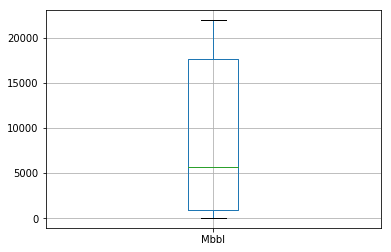
\includegraphics[width=100mm]{oil.png}
	\caption{Number of millions of barrels of oil produced from 1880-1984}
\end{figure}
\\[15mm]
\underline{\textbf{1.11}:} \\ \\
\textbf{(a)} Every year between the dates 67.5 and 69.5, there is one power plant that had an 1100 Megawatt capacity, where others in that time period were mostly between 600 and 900. Also, one power plant constructed at date 71 had capacity of over 1100 Megawatts. When looking at cost compared to the date, we can see that one power plant cost \$90 million whereas the second highest cost was around \$70 million. \\ \\
\textbf{(b)} Mean: \$46.16 million$\hspace{15mm}$ Std: \$17.01 million \\ \\
\textbf{(c)} Mean: 825.375 Megawatts$\hspace{15mm}$ Std: 189.36 Megawatts \\ \\
\textbf{(d)} The histogram (Figure 2) isn't very skewed, probably because as technology increases, so can the capacity of the power plants, but at the same time, technology increasing generally means that the cost decreases.
\\
\begin{figure}[h!]
	\centering
	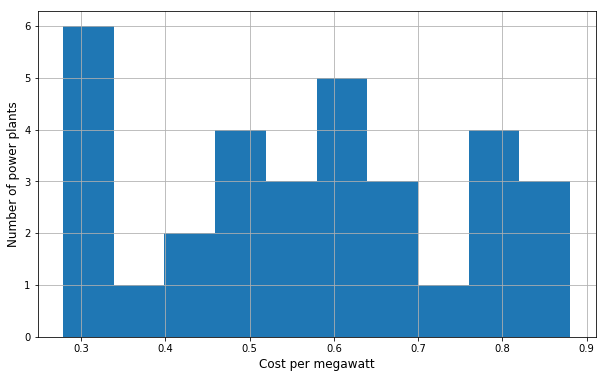
\includegraphics[width=100mm]{cpm.png}
	\caption{Histogram of Cost per Megawatt in power plants}
\end{figure}
\
\\[20mm]
\underline{\textbf{1.12}:} \\ \\
With respect to calories, the histograms for Beef and Poultry had a skew to the right, while the histogram for Meat had a skew to the left. The standard deviations for the calories for all three meats were very similar ($\sim$22-25), and both Beef and Meat had very similar mean calories ($\sim$157), but the mean calories for Poultry was far lower ($\sim$118). \\ \\
In regards to sodium, both the Beef and Poultry histograms had a left skew, while the Meat histgram had a skew to the right. Standard deviations were all in the range 84-102 and means were all within 401-418, which isn't a large percent change.
\begin{figure}[h!]
	\centering
	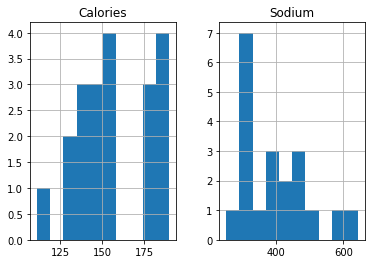
\includegraphics[width=80mm]{beef_hist.png}
	\caption{Histogram of calories and sodium in Beef hotdogs}
\end{figure}
\begin{figure}[h!]
	\centering
	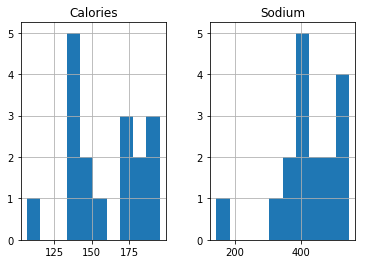
\includegraphics[width=80mm]{meat_hist.png}
	\caption{Histogram of calories and sodium in Meat hotdogs}
\end{figure}
\begin{figure}[h!]
	\centering
	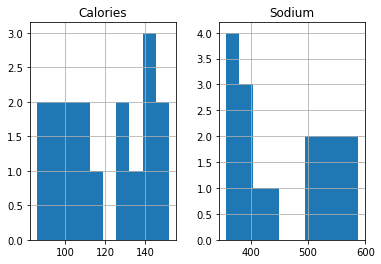
\includegraphics[width=80mm]{poultry_hist.png}
	\caption{Histogram of calories and sodium in Poultry hotdogs}
\end{figure}
\newpage
\ \\
\underline{\textbf{1.13}:} \\ \\
\textbf{(a)} Groups 1 and 2 have a similar box shape, but the mean and total position of box 1 are greater than box 2, which follows an obvious trend that magazines of a higher education level have more 3 syllable words. Group 3 follows this trend in that it has a lower variance (most of the points fall within the 10-15 frequency range) and has a mean less than group 1. Group 3 does have a few outliers, but overall, it looks like group 3 is the group with the least amount of 3 syllable words. \\
\begin{figure}[h!]
  \centering
  \begin{subfigure}[b]{0.4\linewidth}
    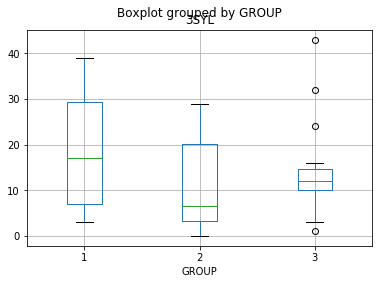
\includegraphics[width=\linewidth]{3syl.png}
    \caption{3 syllable words by\\magazine group}
  \end{subfigure}
  \begin{subfigure}[b]{0.4\linewidth}
    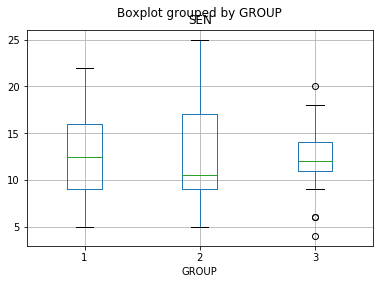
\includegraphics[width=\linewidth]{sen.png}
    \caption{Number of sentences by\\magazine group}
  \end{subfigure}
  \label{fig:coffee}
\end{figure}
\\
\textbf{(b)} In examining the number of sentences, the means are approximately the same across all three groups, but the variances are what differ. The variances for group 1 and group 2 are very similar, but the variance for group 3 is smaller than the others. As with the syllables, group 3 had a few outliers in the number of sentences, this time on the lower end.
\\[20mm]
\underline{\textbf{1.14}:} \\ \\
\textbf{(a)} The distributions seem almost the same, but upon examining the percentiles, the $70^{th}$ percentile of the Math students' drinking during the week was 1.8, in other words, 70\% of the Math students' data was at a 1.8 on a 1-5 scale or lower. This is compared to the Portugese students who had a $70^{th}$ percentile occuring at 2.0 on a 1-5 scale. This means that slightly more Portugese students had a higher rating for drinking during the week.
\begin{figure}[h!]
  \captionsetup{justification=centering}
  \centering
  \begin{subfigure}[b]{0.2\linewidth}
    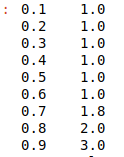
\includegraphics[width=\linewidth]{math_hist.png}
  \end{subfigure}
  \hspace{30mm}
  \begin{subfigure}[b]{0.2\linewidth}
    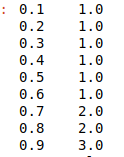
\includegraphics[width=\linewidth]{port_hist.png}
  \end{subfigure}
  \caption{Percentiles of levels of Math (left) and Portugese (right)\\students that drink during the week}
  \label{fig:coffee}
\end{figure} \\ \\
\textbf{(b)} Upon grouping all the data together and only looking at the family size, I was able to determine that those individuals in families 'LE3' or 'Less than or equal to 3' drank on the weekends more than those individuals in the group 'GT3' or 'Greater than 3' members in the family. I was able to determine this by exmaining the histograms, but again confirmed with the percentiles of data. Around 30\% of the 'LE3' data points fall within the 1.0 on the 1-5 scale for drinking while about 40\% of the 'GT3' data points fall within the 1.0. Looking at the other end, about only 80\% of the 'LE3' points fall within the 1.0-4.0 while 90\% of the 'GT3' points fall within the 1.0-4.0 range. I conclude that more students with families less than or equal to 3 tend to drink more on the weekends than students in families of size greater than 3. \\ \\
\begin{figure}[h!]
  \captionsetup{justification=centering}
  \centering
  \begin{subfigure}[b]{0.4\linewidth}
    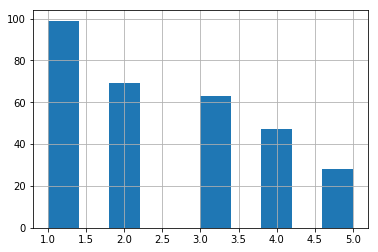
\includegraphics[width=\linewidth]{le3.png}
  \end{subfigure}
  \hspace{10mm}
  \begin{subfigure}[b]{0.4\linewidth}
    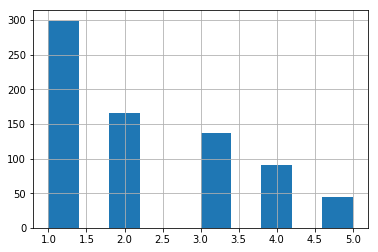
\includegraphics[width=\linewidth]{gt3.png}
  \end{subfigure}
  \caption{Histograms of levels of drinking during the week for LE3 (left) and GT3 (right) students.}
  \label{fig:coffee}
\end{figure}
\begin{figure}[h!]
  \captionsetup{justification=centering}
  \centering
  \begin{subfigure}[b]{0.2\linewidth}
    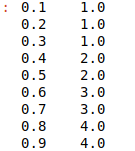
\includegraphics[width=\linewidth]{le3_perc.png}
  \end{subfigure}
  \hspace{30mm}
  \begin{subfigure}[b]{0.2\linewidth}
    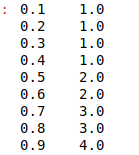
\includegraphics[width=\linewidth]{gt3_perc.png}
  \end{subfigure}
  \caption{Percentiles of levels of drinking during the week for LE3 (left) and GT3 (right students.}
  \label{fig:coffee}
\end{figure}
\\[25mm]
\textbf{(c)} After creating a new column with the weighted average of weekend drinking and weekday drinking, I plotted sixteen different boxplots (Figure 10) of every combination of \{school, sex, famsize, romantic\}. Upon examination, it was obvious that 5 data points had a higher mean than the rest. These groups had a mean total drinking score of 2.0-2.5:
\begin{itemize}
	\item \{GP, M, LE3, yes\}
	\item \{MS, M, GT3, no\}
	\item \{MS, M, GT3, yes\}
	\item \{MS, M, LE3, no\}
	\item \{MS, M, LE3, yes\}
\end{itemize}
\ \\
If we were to generalize these categories, we would see that students going to school at Mousinho da Silveira that were male tend to go out more than other students.
\begin{figure}
	\centering
	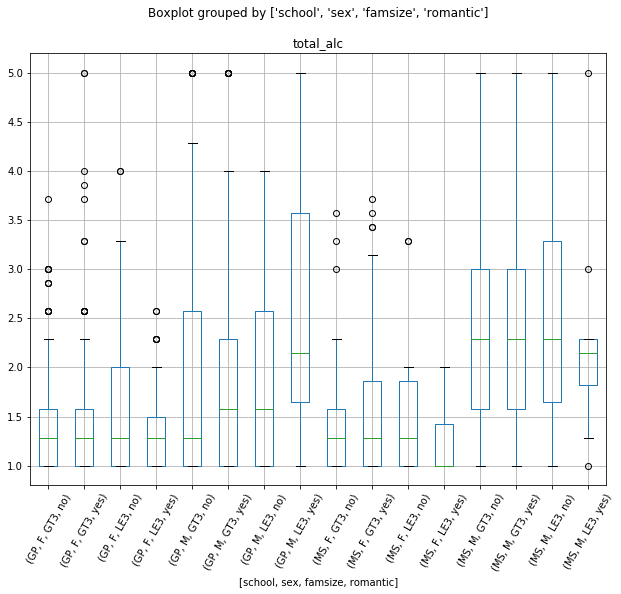
\includegraphics[width=\linewidth]{big_box.png}
	\caption{}
\end{figure}


\end{document}
